\documentclass{article}
        \usepackage{tikz}
        \usepackage{pgfplots}
        \begin{document}
        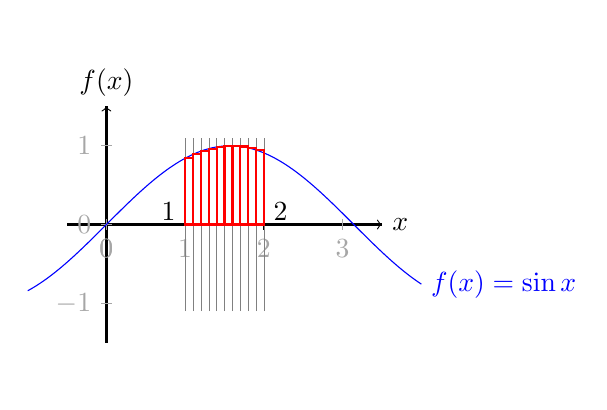
\begin{tikzpicture} [domain = -1:4, scale = 1]
        \clip (-1, -2) rectangle(6, 2.5); 
        \draw[thick](0, -1.5) -- (0, 1.5)node[above]{$f(x)$}; % Oy axis
        \draw[thick](-0.5, 0) -- (3.5, 0)node[right]{$x$}; % Ox axis
        \draw[->](0, 0) -- (0, 1.5); % arrow Oy
        \draw[->](0, 0) -- (3.5, 0);% arrow Ox
    \foreach \x in{0,...,0 }% Ox designation<0
        \draw[gray!70!white](\x cm, 2pt) -- (\x cm, -2pt) node[anchor = north]{$\x$};%dashes on Ox
    \foreach \x in{0,...,3 }% Ox designation>0
        \draw[gray!70!white](\x cm, 2pt) -- (\x cm, -2pt) node[anchor = north]{$\x$};%dashes on Ox
    \draw(2, 2pt) -- (2, -2pt) node[anchor = south west]{2}; % finish dashes
\draw(1, 2pt) -- (1, -2pt) node[anchor = south east]{1}; % start dashes
    \foreach \y in{-1,...,1}% Oy designation
        \draw[gray!70!white](2pt, \y cm) -- (-2pt, \y cm) node[anchor = east]{$\y$};%dashes on Oy

    \draw[blue, samples = 1000]   plot(\x, {sin(\x r) }) node[right]{$f(x) = \sin x$ }; % function

        \foreach \x in{1,1.1,...,2.001 }% lines with steps
        \draw[gray, very thin](\x, -1.1) -- (\x, 1.1);

        \foreach \x in{1,1.1,...,1.999 }% rectangels
        \draw[red, thick](\x, 0) rectangle(\x + 0.1, {sin(deg(\x)) }); 

    \end{tikzpicture}
        \end{document}